\section{Auswertung}
    \subsection{Ätzgrübchendichte}
        Zunächst gilt es die Nominale Unordnung der Proben zu definieren, dies lässt sich über die Ätzgrübchendichte an der Oberfläche
        realisieren. Dazu wurden für beide Proben je 3 Bilder von verschiedenen Positionen an der Oberfläche aufgenommen und anschließend
        aus der Fläche, aufgenommen durch das Mikroskop, und den sichtbaren Ätzgrübchen die Ätzgrübchendichte bestimmt. Dieser Vorgang ist,
        durch das manuelle Zählen der Grübchen sehr müßig und ungenau, lässt aber dennoch eine Qualitative aussage über die Ordnung im Kristall zu.
        Aus den Aufgenommen Bildern lies sich folgende Tabelle erstellen.
        \begin{table}[H]
            \centering
            \begin{tabular}[]{c|c|c|c|c}
                Probe & Aufnahme Nr. & Anzahl Grübchen & Fläche [$\mu m^2$] & Dichte [$\frac{n}{\mu m^2}$] \\
                \hline
                \multirow{3}{*}{\rotatebox[origin=c]{90}{Get.}} & 1 & $39 \pm 3$ & 839908,67 & 4,64e-5 \\
                                                                     & 2 & $25 \pm 3$ & 1099357,61& 2,27e-5 \\
                                                                     & 3 & $31 \pm 3$ & 454314,66 & 6,82e-5 \\
                Mittelwert                                           & - & - & - & $4,58e-5 \pm 2,27$\\
                \hline
                \multirow{3}{*}{\rotatebox[origin=c]{90}{Unget.}}  & 1 & $344 \pm 40$  & 18894,73 & 0,018 \\
                                                                        & 2 & $27 \pm 5$    & 7942,73 & 0,003 \\
                                                                        & 3 & $103 \pm 15$  & 6251,25 & 0,017 \\
                Mittelwert                                           & - & - & - & $0,013 \pm 0,008$\\
                
            \end{tabular}    
        \end{table}
        Es ist deutlich zu erkennen, dass die Ätzgrübchendichte der ungetemperten Probe um ein Vielfaches höher ist, als die der getemperten.
        Auch ist zu erkennen, dass die Ätzgrübchendichte an verschiedenen stellen der Oberfläche stark variiert, also nicht konstant ist.
    \begin{figure}[H]
        \centering
        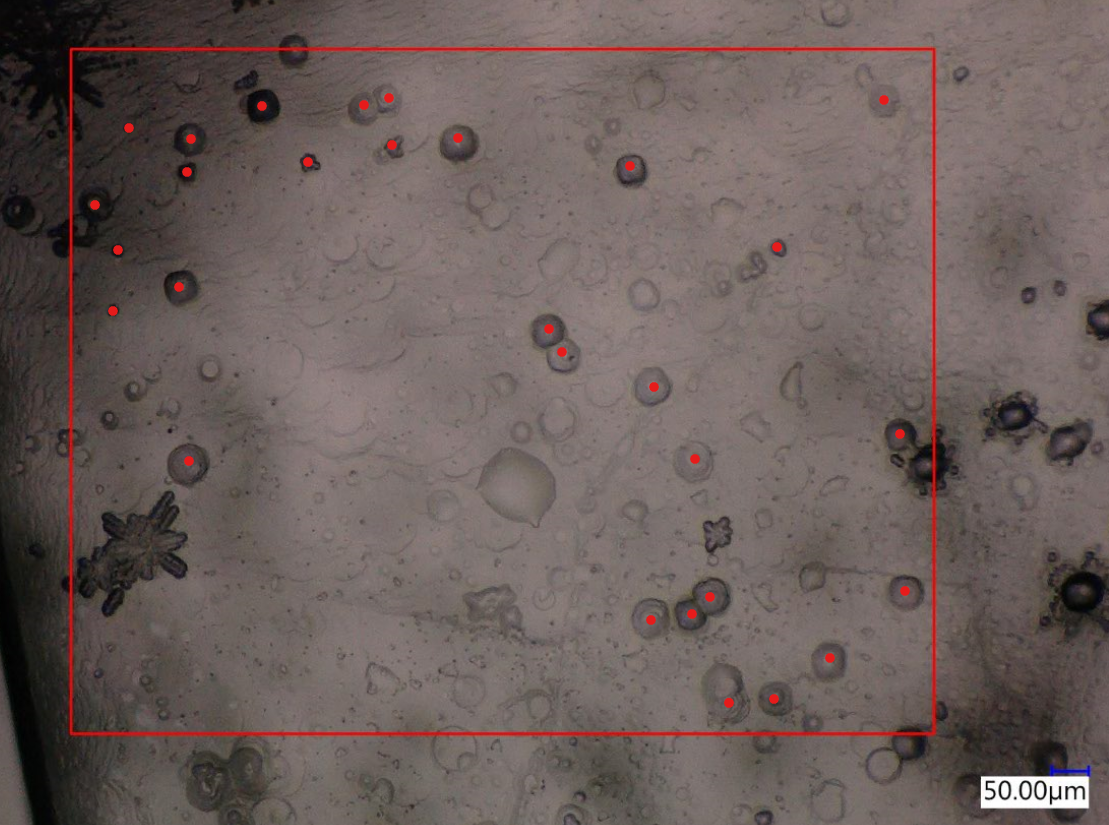
\includegraphics[width=\textwidth]{Images/Beispiel_ätzgrübchendichte.PNG}
        \caption{Beispiel einer Aufnahme für die Ätzgrübchendichte.}
    \end{figure}

    \subsection{Kleinwinkelkorngrenzen}
        \subsubsection*{Rosetten durch Nadeleindruck}
            Im Anschluss an die Bestimmung der Ätzgrübchendichte wurde auch ein Bild einer vermutlichen Kleinwinkelkorngrenzen aufgenommen, um aus diesem
            den Winkel zwischen den Kristalliten zu bestimmen. Um den Winkel aus den Abständen zwischen den Ätzgrübchen zu bestimmen wurde bereits in der Vorbereitung
            folgende Formel hergeleitet
            \begin{equation}
                \theta = \arctan(\frac{b}{d}) \approx \frac{b}{d} \approx \frac{n\cdot a}{\sqrt{2}\cdot d}
            \end{equation}
            Wobei $n$ die Anzahl der Ätzgrübchen angibt und $d$ den abstand zwischen dem ersten und letzten. Zudem nehmen wir für $b=\frac{a}{\sqrt{2}}$ an, sodass für
            Messungen mit mehreren Grübchen ein gesamt Verschiebung von $b_ges = n * g$ gilt.
            Mit folgender Aufnahme
            \begin{figure}[H]
                \centering
                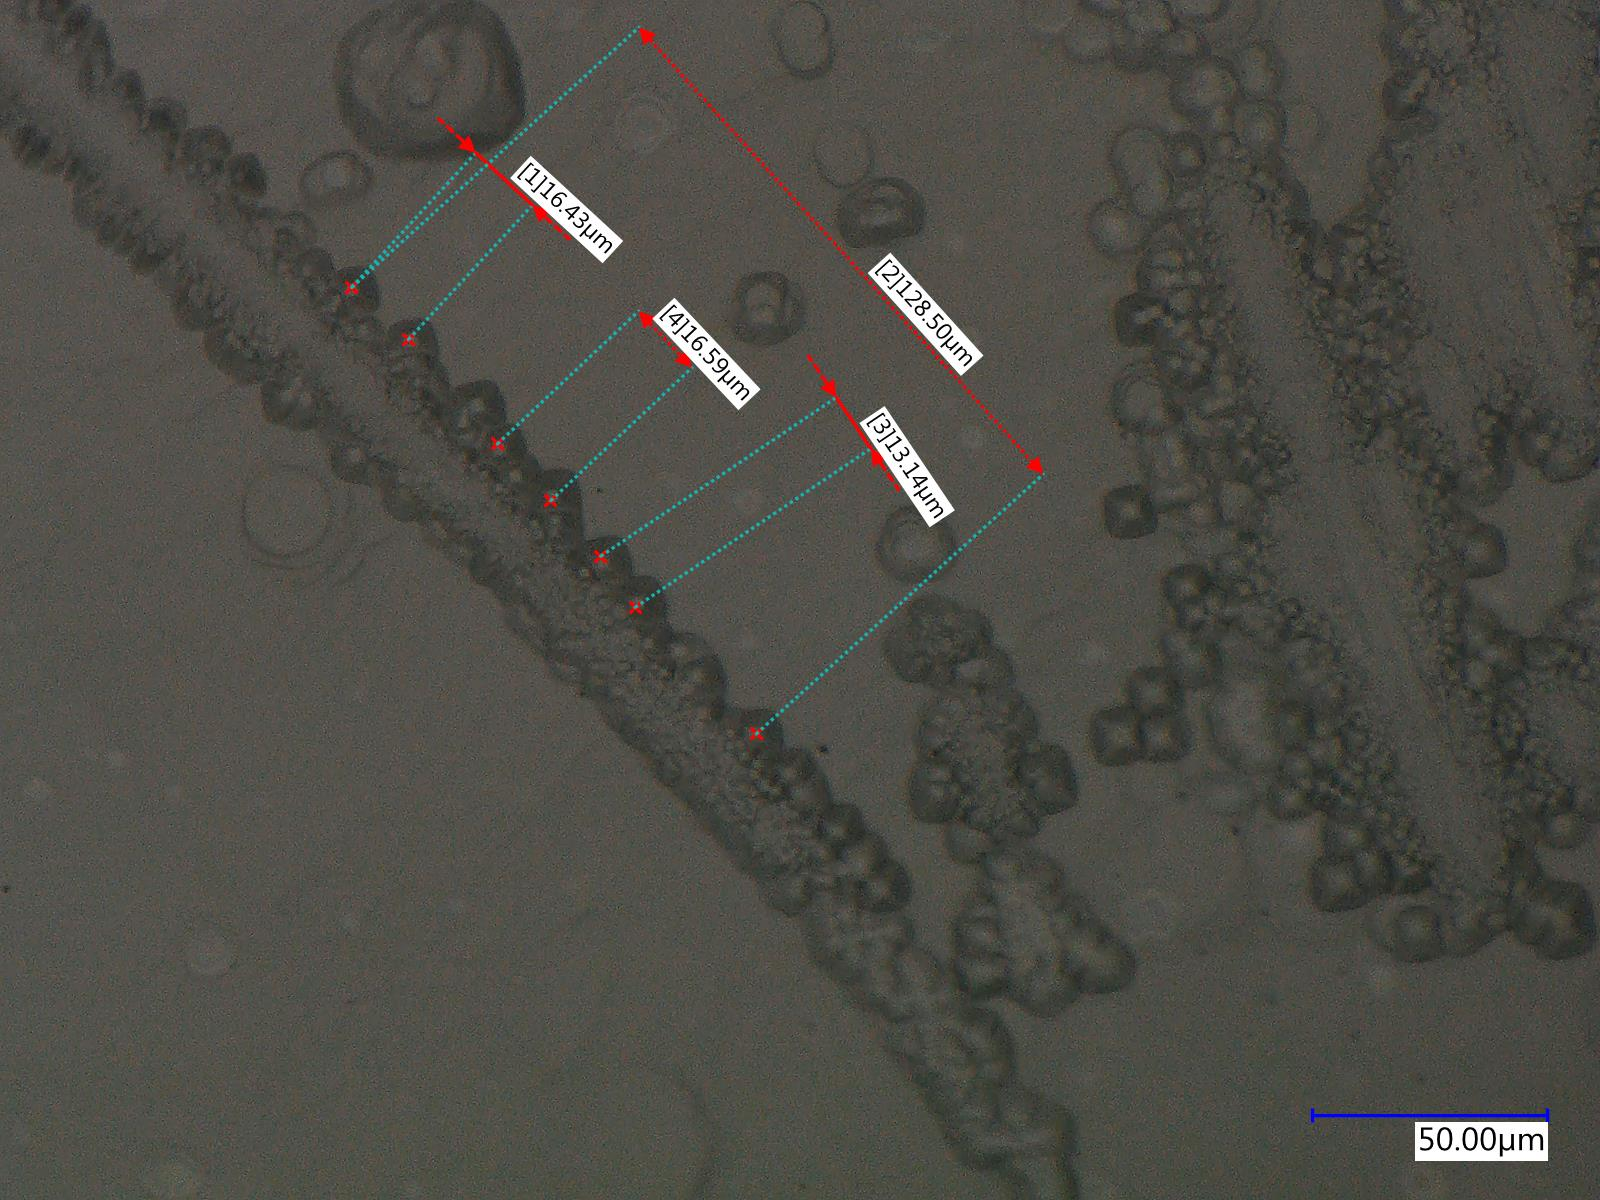
\includegraphics[width=\textwidth]{Images/kleinwinkelkorngrenze 2.jpg}
                \caption{Aufnahme einer vermutlichen Kleinwinkelkorngrenzen mit Abständen}
            \end{figure}
            Konnte folgende Tabelle erstellt werden
            \begin{table}[H]
                \centering
                \begin{tabular}[]{c|c|c}
                    Abstand d [$\mu m$] & Anzahl Grübchen n & Winkel $\theta$ [°] \\
                    \hline
                    $128,5 \pm 1$ & 9 & $1,14e-3 \pm 1,55e-10$\\
                    $16,43 \pm 1$ & 1 & $0,99e-3 \pm 1,05e-9$\\
                    $16,59 \pm 1$ & 2 & $1,96e-3 \pm 2,07e-9$\\
                    $13,14 \pm 1$ & 1 & $1,24e-3 \pm 1,65e-9$\\   
                \end{tabular}
            \end{table}
            Grundsätzlich entsprechen die Winkel den Erwartungen, da diese recht klein ausfallen, jedoch lässt die Messmethode nur ganzzahlige n zu, die nur eine
            geringe Auflösung der Tatsächlichen abstände d zulassen.
        \subsection{Versetzungsbewegungen}
            Dieser abschnitt befasst sich mit der Wanderung der der Versetzungen bei äußerer Druckeinwirkung, dazu wurden 2-3 Rosetten durch Nadeleindruck erzeugt,
            deren Dimension über das Mikroskop aufgenommen und anschließend durch axialen Druck bewegt. Durch das Gewicht der Presse sowie der Querschnittsfläche der Probe
            lässt sich die Kraft bestimmen und über die Dauer der Anwendung die Geschwindigkeit der Wanderung.
            \begin{figure}[H]
                \begin{minipage}[b]{.4\linewidth} % [b] => Ausrichtung an \caption
                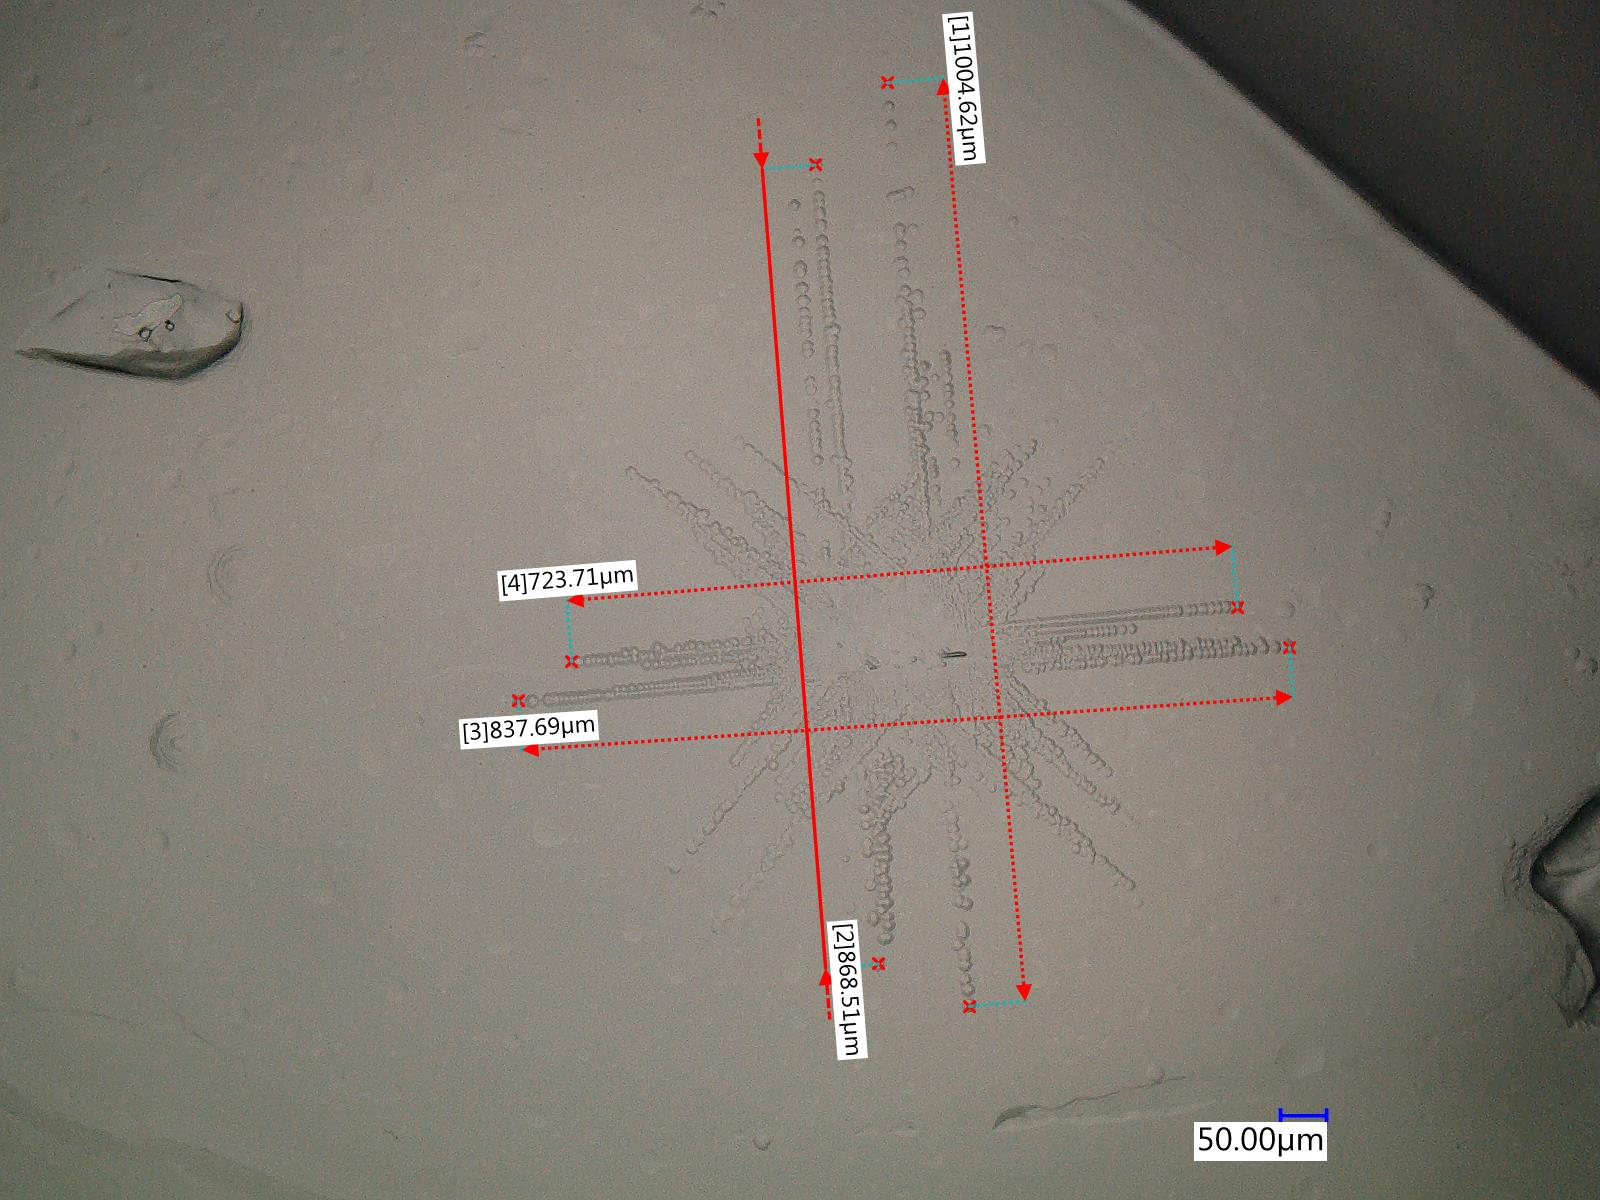
\includegraphics[width=\linewidth]{Images/eriks rosette 1 messung A.jpg}
                \end{minipage}
                \hspace{.1\linewidth}% Abstand zwischen Bilder
                \begin{minipage}[b]{.4\linewidth} % [b] => Ausrichtung an \caption
                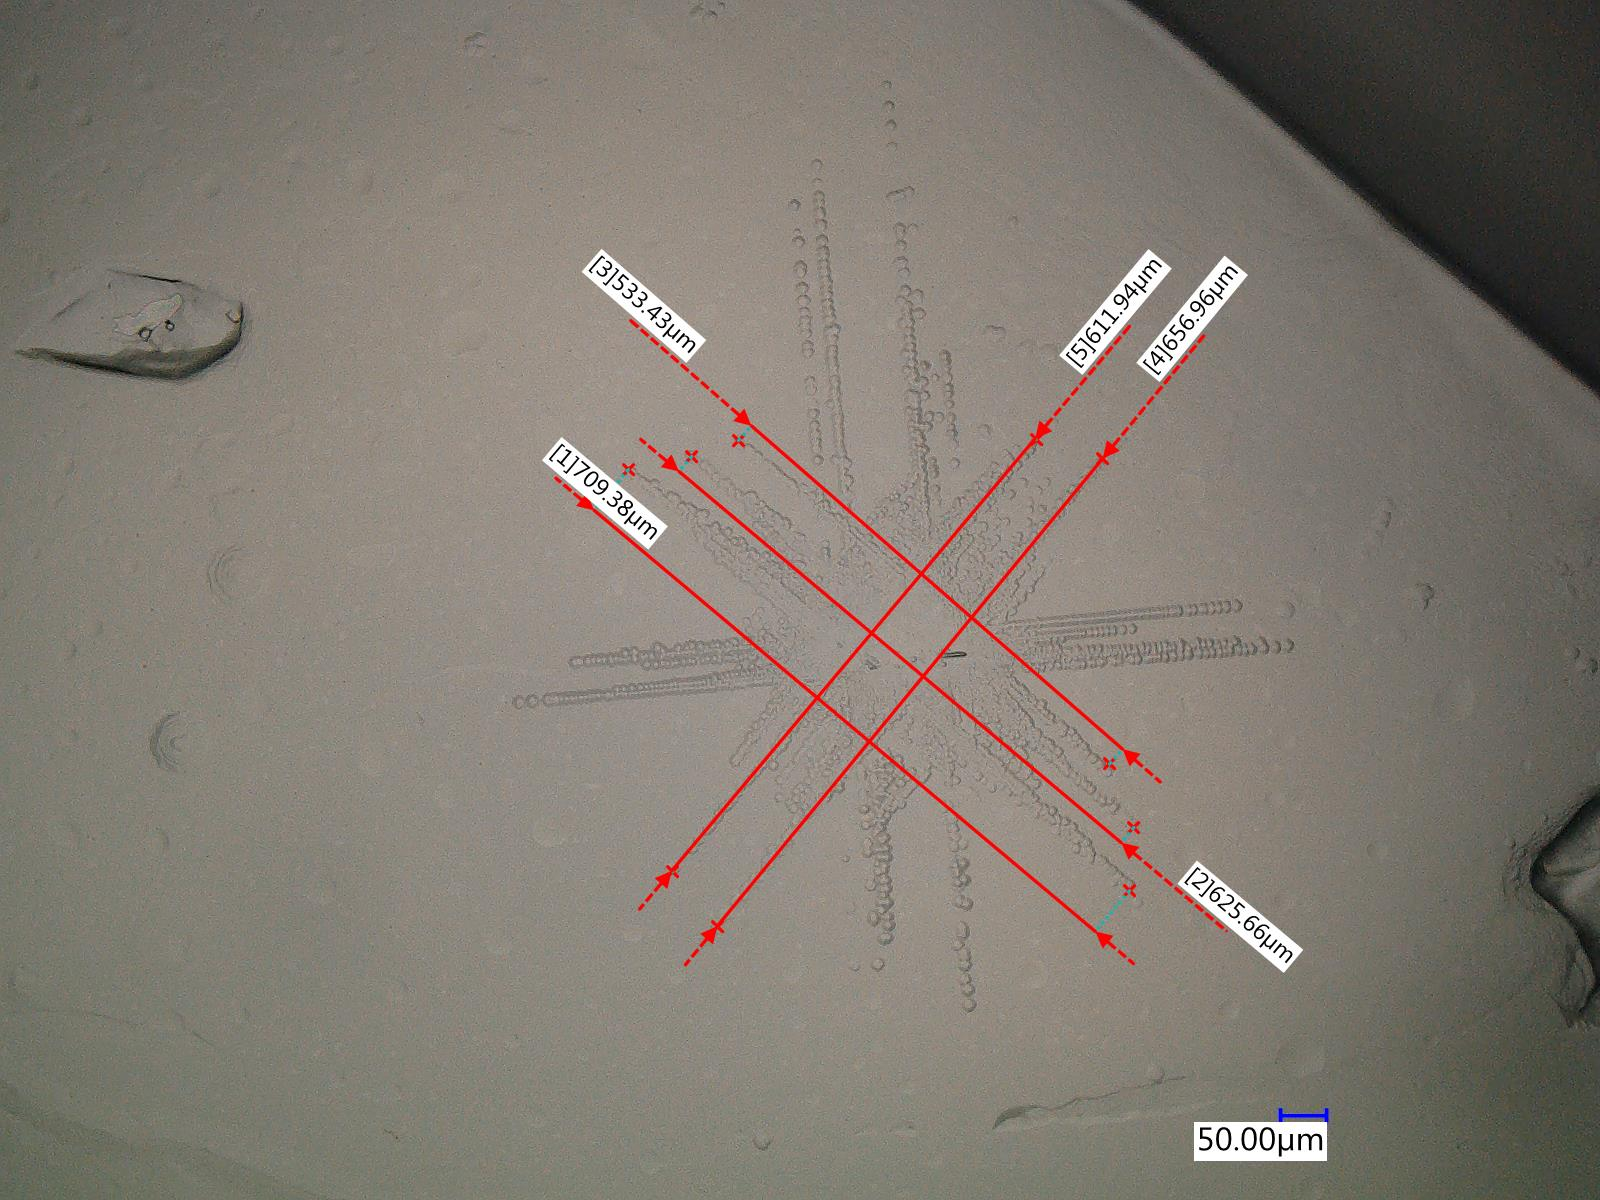
\includegraphics[width=\linewidth]{Images/eriks rosette 1 messung B.jpg}
                \end{minipage}
                \caption{Aufnahme eines Nadeleindrucks mit Abmessungen vor der Anwendung des Axialen Drucks}
            \end{figure}
            \begin{figure}[H]
                \centering
                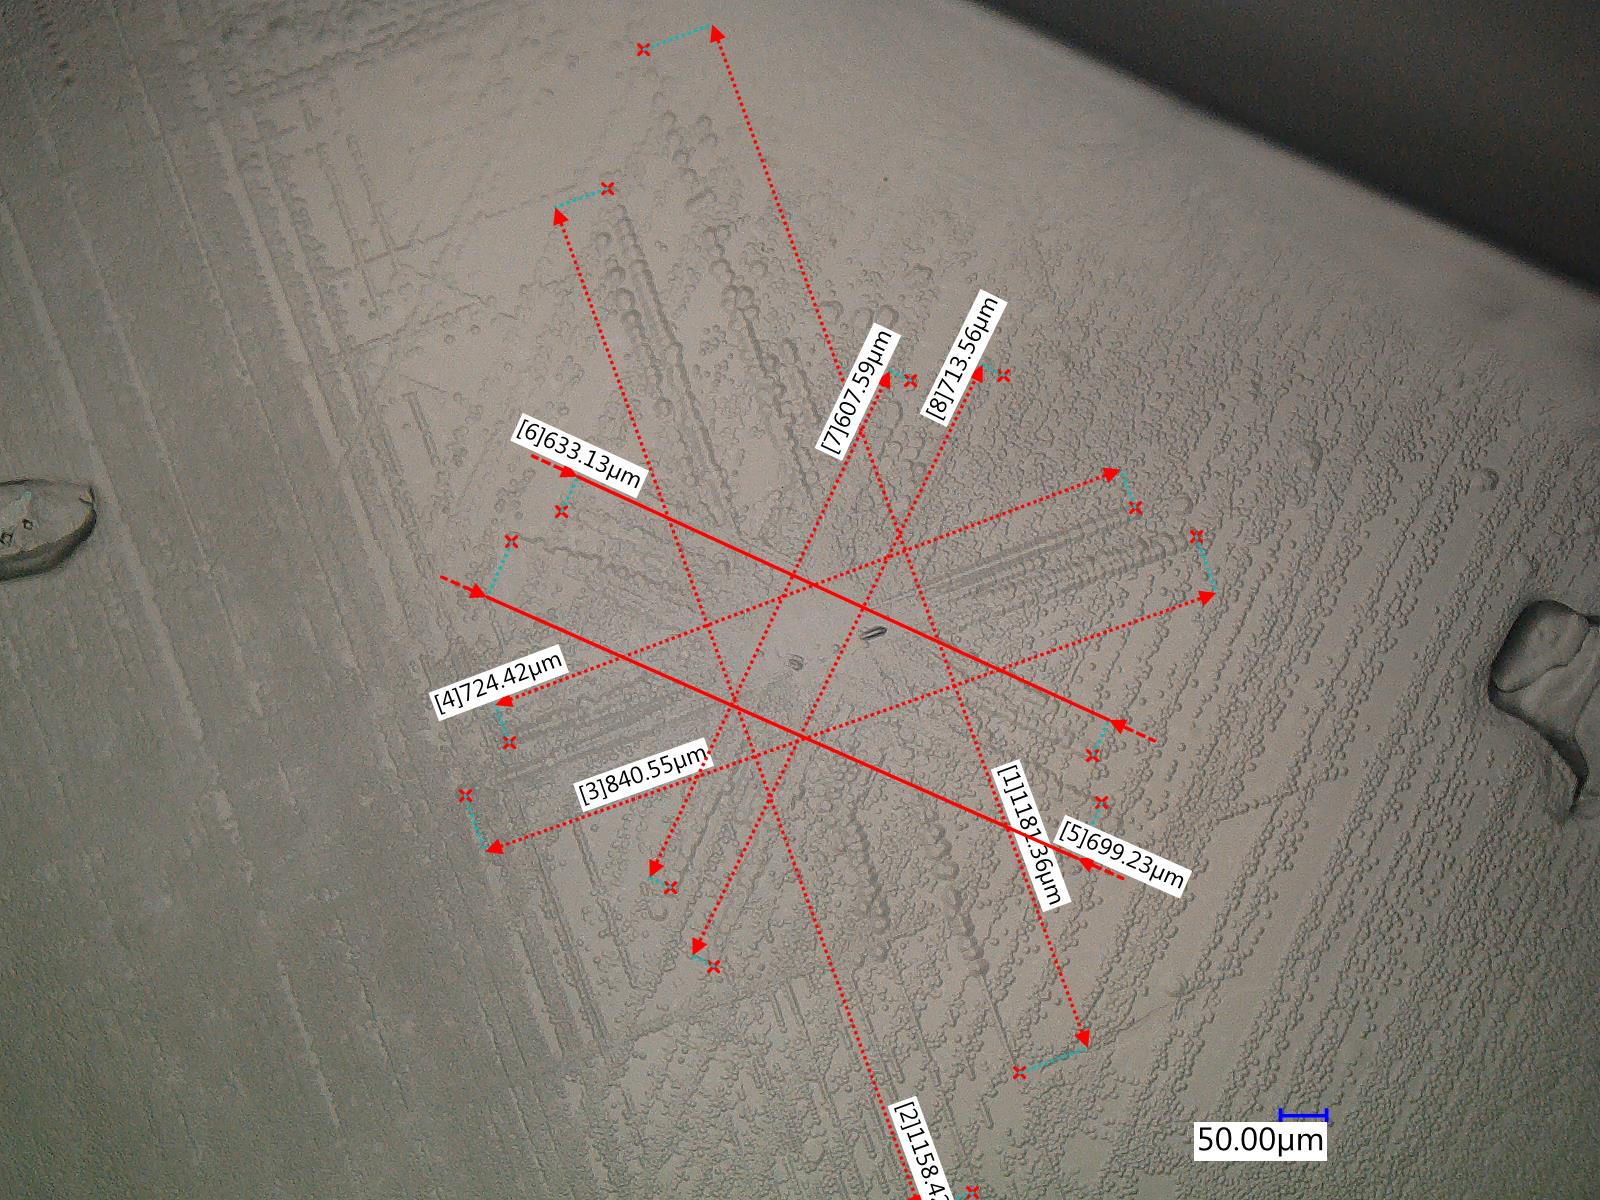
\includegraphics[width=\linewidth]{Images/eriks rosette 1PD Messung.jpg}
                \caption{Aufnahme eines Nadeleindrucks mit Abmessungen nach der Anwendung des Axialen Drucks}
            \end{figure}
            Aus den Messungen durch das Mikroskop lassen sich grob folgende Messungen für die Wanderungsdistanz bestimmen
            \begin{table}[H]
                \centering
                \begin{tabular}[]{c|c|c|c}
                    Vorher [$\mu m$] & Nachher [$\mu m$] & Differenz [$\mu m$] & Geschwindigkeit [$\frac{\mu m}{min}$] \\
                    \hline
                    $837,69 \pm 5$  & $840,55 \pm 5$    & $ 2,8 \pm 10$     & $0,95 \pm 3,33$ \\
                    $723,71 \pm 5$  & $724,42 \pm 5$    & $ 0,71 \pm 10$    & $0,24 \pm 3,33$ \\
                    $868,51 \pm 5$  & $1158,42 \pm 5$   & $ 289,91 \pm 10$  & $96,64 \pm 8,72$\\
                    $1004,62 \pm 5$ & $1181,36 \pm 5$   & $ 176,74 \pm 10$  & $58,91 \pm 5,93$\\
                    $533,43 \pm 5$  & $633,13 \pm 5$    & $ 99,7 \pm 10$    & $33,23 \pm 4,33$\\
                    $709,38 \pm 5$  & $699,23 \pm 5$    & $ -10,15 \pm 10$  & $-3,38 \pm 3,35$\\
                    $611,94 \pm 5$  & $607,59 \pm 5$    & $ -4,35 \pm 10$   & $-1,45 \pm 3,34$\\
                    $656,96  \pm 5$ & $713,56  \pm 5$   & $ 56,6 \pm 10$    & $18,87 \pm 3,69$\\
                \end{tabular}
                \caption{Messung der Wanderung der Rosettenarme}
            \end{table}
            Es ist deutlich zu erkennen, dass durch den axialen Druck nur wenige Arme, die entlang der <110> Richtung, ein Starkes Wachstum erfahren haben, das Wachstum der anderen Arme ist im Rahmen unsere
            Messgenauigkeit kaum aussagekräftig, ließe sich jedoch auf die Statistische Verteilung der Energie entlang aller Achsen zurückführen.
        \subsubsection*{Schubspannung im Gleitsystem}
            Um den Druck im Gleitsystem zu bestimmen wurde das angewandte Gewicht ($g = 2,716 Kg$) der Presse sowie die Druckfläche ($A=3618962,9 \mu m^2$)der Probe bestimmt.
            Mit
            \begin{equation}
                F = m \cdot a = 26,64 N
            \end{equation}
            folgt die Kraft und anschließend über
            \begin{equation}
                \sigma = F / A = 736,23e4 \frac{N}{m}
            \end{equation}
            Die Schubspannung.